\clearpage
\section{Quantum Oblivious Key Distribution with Discrete Variables}

\begin{tcolorbox}	
\begin{tabular}{p{2.75cm} p{0.2cm} p{10.5cm}} 	
\textbf{Student Name}  &:& Mariana Ramos\\
\textbf{Starting Date} &:& September 18, 2017\\
\textbf{Goal}          &:& Quantum oblivious key distribution (QOKD) implementation with discrete variables.
\end{tabular}
\end{tcolorbox}

Oblivious Transfer (OT) is a fundamental primitive in multi-party computation. The one-out-of-two OT consists in a communication protocol between Alice and Bob. At the beginning of the protocol Alice has two messages $m_1$ and $m_2$ and Bob wants to know one of them, $m_b$, without Alice knowing which one, i.e. without Alice knowing $b$, and Alice wants to keep the other message private, i.e. without Bob knowing $m_{\bar{b}}$. therefore two conditions must be fulfilled:
\begin{enumerate}
	\item{The protocol must be concealing, i.e at the beginning of the protocol Bob does not know nothing about Alice's messages, while at the end of the protocol Bob will learn the message $m_{b}$ chosen by him.}
	\item{The protocol is oblivious, i.e Alice cannot learn anything about Bob's choice, bit $b$, and Bob cannot learning nothing about the other message $m_{\bar{b}}$.}
\end {enumerate}

In order to implement OT between two parties (Alice and Bob) they must be able to exchange continuously oblivious keys, i.e a QOKD system must exist between them.

\subsection{QOKD system}

In this section we are going to describe the quantum oblivious key distribution system.

Considering a discrete variables implementation, both Alice and Bob agree with the following correspondence, where $+$ corresponds to \textit{Rectilinear Basis} and $\times$ corresponds to \textit{Diagonal Basis},

\begin{table}[H]
\centering
\begin{tabular}{c|c}
\textbf{\textit{Basis}}         &  \\ \hline
 0 & $+$ \\
 1 & $\times$ \\
\end{tabular}
\end{table}
Alice and Bob also agree with the bit correspondence for each direction for each basis. For \textit{Rectilinear basis}, "$+$",

\begin{table}[H]
\centering
\begin{tabular}{c|c}
            & Basis "+" \\ \hline
 0 & $\to (0^{\circ})$ \\
 1 & $\uparrow (90^{\circ})$ \\
\end{tabular}
\end{table}
and for \textit{Diagonal Basis}, "$\times$",

\begin{table}[H]
\centering
\begin{tabular}{c|c}
      & Basis "$\times$" \\ \hline
 0 & $\searrow (-45^{\circ})$ \\
 1 & $\nearrow (45^{\circ})$ \\
\end{tabular}
\end{table}

\begin{enumerate}
  \item The first step is to establish for both Alice and Bob the block length $l$. In this case, lets assume $l=16$. Alice randomly generate a bit sequence with length $l$.
      Therefore, she must define two sets randomly: $S_{A1}$ which contains the basis values; and $S_{A2}$, which contains the key values.

      In that case, lets assume she generates the following sets $S_{A1'}$ and $S_{A2'}$:
      $$S_{A1'} = \{0,0,1,1,1,0,0,1,1,0,0,1,1,1,0,1 \},$$
      $$S_{A2'} = \{1,1,1,0,0,0,0,0,1,1,0,0,1,0,1,1 \}.$$

  \item Next, Alice sends to Bob throughout a quantum channel $l$ photons encoded using the basis defined in $S_{A1'}$ and according to the key bits defined in $S_{A2'}$.

      Therefore, in the current example, Alice sends the following photons,

      \begin{align*}
        S_{AB} & = \{\uparrow,\uparrow, \nearrow, \searrow, \searrow, \to, \to, \searrow, \nearrow,\uparrow, \to, \searrow,\nearrow,\searrow,\uparrow,\nearrow \} \\
          & =\{90^{\circ},90^{\circ}, 45^{\circ}, -45^{\circ},-45^{\circ}, 0^{\circ}, 0^{\circ}, -45^{\circ}, 45^{\circ},90^{\circ}, 0^{\circ}, -45^{\circ}, 45^{\circ}, -45^{\circ}, 90^{\circ}, 45^{\circ} \}.
        \label{eq:photonsalice}
      \end{align*}


  \item Bob also randomly generates $l=16$ bits, which are going to define his measurement basis, $S_{B1'}$. Lets assume,
        \begin{align*}
             S_{B1'} & = \{0,1,1,0,0,1,0,1,1,0,1,1,0,0,0,1 \} \\
                    & = \{ +,\times,\times,+,+,\times,+,\times, \times,+, \times, \times \,+,+,+,\times \}.
        \end{align*}

      Bob will get $l$ results:
      $$S_{B2'} = \{1,-,\underline{0},0,-,1,\underline{1},-,1,-,1,0,1,1,\underline{0},1 \}.$$

      The $'-'$ corresponds to no clicks in Bob's detector. These no clicks happen due to attenuation. The underlined values are bits which were measured with a correct basis but an error has occurred.

  \item Bob is going to send a $'-1'$ or a hash value to Alice for each measurement that he performed, thereby being $'-1'$ the measurements which correspond to no clicks. In this case, we are going to assume that the hash value is calculated using the \textit{SHA-256} algorithm \cite{Liu2009}. In detail, Bob has two sets $S_{B1'}$ and $S_{B2'}$ and he is going to generate the set $S_{BH1}$ which have $l$ hash values calculated for each position of $S_{B1'}$ with the correspondent position of $S_{B2'}$. Therefore, Bob will send to Alice the following set:
      $$S_{BH1}=\{{sha}_{1},-1,{sha}_{2},{sha}_{3}, -1,{sha}_{4},{sha}_{5},-1,{sha}_{6},-1,{sha}_{7},{sha}_{8},{sha}_{9},{sha}_{10},{sha}_{11},{sha}_{12} \}.$$


  \item Since Alice has received the confirmation of measurement from Bob, i.e after Alice has received $S_{BH1}$, she sends throughout a classical channel the basis which she has used to codify the photons, which in this case we assumed $S_{A1'} = \{0,-1,1,1,-1,0,0,-1,1,-1,0,1,1,1,0,1 \}$.

      Due to attenuation, the previous sets are reduced to the length $l=12$ and they shall be replaced by the following:
      $$S_{A1}=\{0,1,1,0,0,1,0,1,1,1,0,1 \},$$
      $$S_{A2}=\{1,1,0,0,0,1,0,0,1,0,1,1 \},$$
      $$S_{B1}=\{0,1,0,1,0,1,1,1,0,0,0,1 \},$$
      $$S_{B2}=\{1,\underline{0},0,1,\underline{1},1,1,0,1,1,\underline{0},1 \}$$

  \item In order to know which photons were measured correctly, Bob does the operation $S_{B3}=S_{B1} \oplus S_{A1}$.
      In the current example the operation will be:

  \begin{table}[H]
    \centering
    \begin{tabular}{c|c c c c c c c c c c c c }
     $S_{B1}$ & 0 & 1 & 0 & 1 & 0 & 1 & 1 & 1 & 0 & 0 & 0 & 1\\
     $S_{A1}$ & 0 & 1 & 1 & 0 & 0 & 1 & 0 & 1 & 1 & 1 & 0 & 1\\ \hline
     $\oplus$ & 1 & 1 & 0 & 0 & 1 & 1 & 0 & 1 & 0 & 0 & 1 & 1
    \end{tabular}
    \end{table}

      In this way, Bob gets $$S_{B3} = \{1,1,0,0,1,1,0,1,0,0,1,1 \}.$$ When Bob uses the right basis he gets the values correctly, apart from possible errors in transmission, when he uses the wrong basis he just guess the value. The values ``$1$'' correspond to the values he measured correctly and ``$0$'' to the values he just guessed.
      Thus, Bob is building two sets of keys, one $'r'$ with correct measurements values and other $'w'$ with the measurement values that he just guessed.

      Thus, Bob has two pair of sets, one for the photons he measured correctly,

      $$S_{B_{rp}}= \{1,2,5,6,8,11,12 \},$$ $$ S_{B_{rb}} = \{1,0,1,1,0,0,1 \},$$
      where $S_{B_{rp}}$ is the set of positions he was right about and $SB_{rb}$ is the set of bit values he measured for each position he was right about. The other pair is for photons he just guessed the measurement,
      $$S_{B_{wp}}= \{3,4,7,9,10 \},$$ $$S_{B_{wb}} = \{0,1,1,1,1 \},$$
      where $S_{B_{wp}}$ is the set of positions he just guessed the values and $S_{B_{wb}}$ is the set of bit values he measured for each position he just guessed the values.

      Nevertheless, due to errors in transmission, some of the bits in $S_{B_{rb}}$ may be not right.

      At this point, in order to test Bob's honesty, Alice is going to ask Bob to open some pairs of the right set and some pairs of the wrong set. These pairs are destroyed from them sets. Lets assume she asked to open two pairs of the right set and one pair of the wrong set. She verified these pairs using the hash function committed by Bob and concluded that he is being honest.

      Now, Bob has the previous sets replaced by the following,
      \begin{align*}
        S_{B_{rp}} & = \{1,2,5,6,8 \} \\
        S_{B_{rb}} & = \{1,0,1,1,0 \} \\
        S_{B_{wp}} & = \{3,4,7,9 \} \\
        S_{B_{wb}} & = \{0,1,1,1 \}
      \end{align*}


      Bob and Alice are going to use a modified version of \textit{Cascade algorithm} to correct the errors due transmission.

      \subsubsection{Modified version of Cascade Algorithm}
      The Cascade algorithm is often used with a key set where all values are supposed right. In this case, Bob has two pairs of sets, one with the position and bit values of photon he measured with the correct basis and other with position and bit values of photon he measured with the wrong basis. He only needs to apply the Cascade algorithm in the set that he measured the photons correctly \cite{Brassard1994}. However, he must apply a modified version of the Cascade in the other set in order to keep in secret from Alice which set corresponds to right and which set corresponds to wrong measurements.

      \begin{enumerate}
        \item Bob randomly generates a bit value. If he gets $0$, he will send to Alice the set $\{ S_{B_{rp}}, S_{B_{wp}}\}$. Otherwise, if he gets $1$ he will send the set $\{S_{B_{wp}}, S_{B_{rp}}\}$. This guarantee that Alice does not know which is the right or wrong set. Lets assume this random bit is "1" and he sends $\{S_{B_{wp}}, S_{B_{rp}}\}$. Lest assume Alice and Bob have agreed with $N=2$, where $N$ is the number of sub-blocks they will firstly divide the original set. After the first iteration, if there still be errors, $N$ will be incremented by 1 for the next iteration. However, if there is some set which Bob thinks is already corrected, this block is discarded and the remaining blocks are divided again.
            If the set to be corrected has a odd number of bits, Bob and Alice must add an additional bit $0$ at the end.

            \label{itema}

        \item Now, Bob applies the Cascade algorithm in the two sets. However, to the wrong set he is going to apply a modified version, the \textit{fake Cascade} in order to hiding that it is the set with wrong positions. In this case, he starts from the modified version of Cascade.

        \item In this modified version Bob generates a random number to define $i$ which is the number of iterations. Assuming $s$ as the size of the set, $i$ must be $ 2 \geq i \leq s $.
            As normal Cascade, in this modified version Bob divide the set in $N$ blocks, where $N$ is agreed with Alice at the beginning of the procedure and $N\geq1$. Lets assume $N=1$. After that, Alice sends to Bob the set with parity of the $N$ blocks. He receives the set and do nothing with it. Bob says to Alice that an error has occurred and $N$ is being incremented until $N \leq \frac{s}{2}$ or until the number of iterations achieves $i$. Bob has been asking Alice for parities to keep her entertained during $i$ iterations.

        \item Bob acknowledge Alice that all values were fixed.

        \item Next, Bob starts to apply the normal Cascade to the right set. Lets assumed they were agreed with first $N=2$.

            \begin{figure}[h]
            	\centering
            	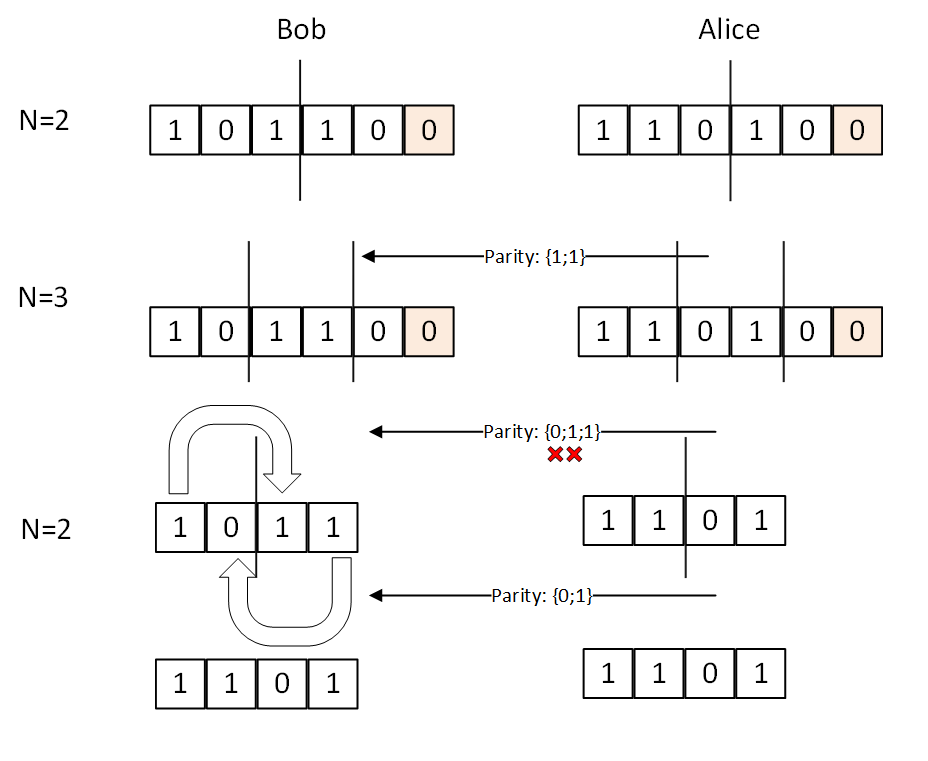
\includegraphics[width=0.7\textwidth, height=7cm]{./sdf/ot_with_discrete_variables/figures/cascade.png}
                	\caption{Cascade algorithm applied in the set of right values.}\label{cascade}
            \end{figure}

            They start with $N=2$ and Alice sends the parity set. After that, as there is a possibility of error, Bob increments for $N=3$ and asks Alice to do the same. After that, Bob discard the last block since the parity matches with Alice's parity. With the other two blocks he change the bits position and combines the first bits and the second bits of each block and he asks Alice for the parity values again.

            By analysing figure \ref{cascade}, the set of right positions is corrected and it will be replaced by the following:

            \begin{align*}
              S_{B_{rp}} & = \{1,2,5,6,8 \} \\
              S_{B_{rb}} & = \{1,1,0,1,0 \} \\
            \end{align*}

      \end{enumerate}


   \item Next, Bob calculates the minimum number between ``ones'' and ``zeros'' in $S_{B3}$, i.e $$n=min(\#0,\#1)=4,$$ where $\#0$ represents the number of zeros in $S_{B2}$ and $\#1$ the number of ones in $S_{B2}$. Bob sends to Alice, throughout a classical channel, the set ${4,w}$, where $4$ is the $n$ and $w$ represents the nature of $n$, i.e in this case $n$ corresponds to the number of wrong measured photons.

  \item When Alice sends to Bob a photons set, they are building a set of pairs (array positions and bit values which correspond to measured photons at Bob's side and to the key bit with the photon was encoded at Alice's side).
      The main goal is to guarantee that Bob has the same number of right and wrong pairs. In addition, they must know information about $t$ (represented in figure \ref{alicebobkeys}) which corresponds to the points where the previous condition is verified.

      Since Bob has sent to Alice the information about the smallest set, in this example, Alice know that there are four pairs of wrong positions and five pairs of right positions. Alice must destroy one of the right pairs by asking Bob to open it. Therefore, at $t=8$ both know that there are the same number of right and wrong pairs thereby being the main goal guaranteed.

    \begin{figure}[h]
    	\centering
    	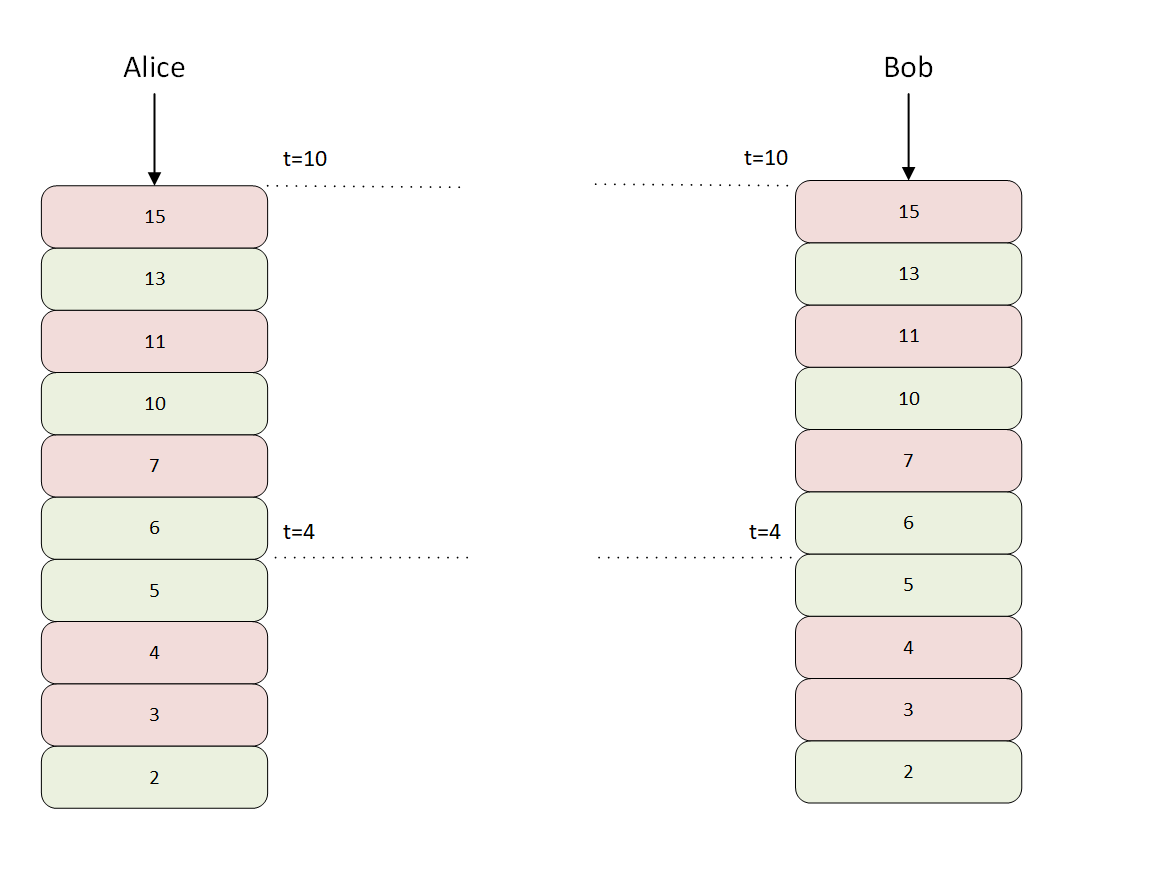
\includegraphics[width=1.0\textwidth, height=9cm]{./sdf/ot_with_discrete_variables/figures/alicebobkeys.png}
        	\caption{Alice and Bob key sets.}\label{alicebobkeys}
    \end{figure}

     As we can see in figure \ref{alicebobkeys}, unlike Bob, Alice does not know which positions corresponds to right or wrong measurements performed by Bob.
     They have been building these sets during all protocol.
\end{enumerate}

\subsection{OT Protocol with QOKD system}
    At this time, we are going to describe the oblivious transfer protocol with detail. As it was referred at the beginning, Alice sends two messages to Bob and he wants to know one of them. Alice does not know which message Bob wants and Bob only know the message he wants, i.e he does not know anything about the other message.
    Furthermore, only Alice knows information about messages $m_{0}$ and $m_{1}$.
    In this case, lets assume the following two messages with size $s=4$, $m_{0} = \{0 0 1 1\}$ and $m_{1} = \{0 0 0 1\}$.
    Alice must guarantee $t = s \times 2$. In order to do that, she must destroy the remaining pairs. In this case, there is no need to do that because they have a set for $t=8$ with the same number of wrong and right pairs.

  \begin{enumerate}
  \item Bob defines two new sub-sets, $I_{0}$ and $I_{1}$. $I_{0}$ is a set of values with photons array positions which Bob just guessed the measurement since he did not measure them with the same basis as Alice, $I_{1}$ is a set of values with photons array positions which Bob measured correctly since he used the same basis as Alice used to encoded them. The position of the pairs of each right and wrong message are in the keys sets that they have been building during the protocol.

  In this example, the message size is 4. Since, at this time $t=10$ and we have $5$ right pairs and $5$ wrong pairs, Alice ask to Bob to open one right pair and one wrong pair in order to both have exactly the message's size number of right and wrong pairs. Lets assume that Alice opened two pairs, position $15$ which is a wrong measurement and position $10$ which is a right measurement. We have now $t=8$.

  Next, Bob defines two sub-sets with size $s=4$:
  $$I_{0}=\{3,4,7,9 \},$$
  and $$I_{1}= \{1,2,6,8 \},$$ where $I_{0}$ is the sequence of positions in which Bob was wrong about basis measurement and $I_{1}$ is the sequence of positions in which Bob was right about basis measurement. Bob sends to Alice the set $S_{b}$

  Thus, if Bob wants to know $m_{0}$ he must send to Alice throughout a classical channel the set $S_{0}=\{I_{1},I_{0} \}$, otherwise if he wants to know $m_{1}$ he must send to Alice throughout a classical channel the set $S_{1}=\{I_{0},I_{1} \}$.


  \item Alice is sure about Bob's honesty, since she knows he only has $4$ right basis to measure the photons. In addition, Alice cannot know which message Bob chose because she did not know the order that he sent the sets.

  \item Lets assume Bob sent $S_{0}=\{I_{1},I_{0} \}$.
   Alice defines two encryption keys $K_{0}$ and $K_{1}$ using the values in positions defined by Bob in the set sent by him. In this example, lets assume: $$K_{0}=\{1,1,1,0\}$$ $$K_{1}=\{0,0,0,1\}.$$

   Alice does the following operations:
   $$m = \{m_{0}\oplus K_{0}, m_{1} \oplus K_{1} \}.$$

   \begin{table}[H]
    \centering
    \begin{tabular}{c|c c c c c c c c}
     $m_{0}$ & 0 & 0 & 1 & 1 \\
     $K_{0}$ & 1 & 1 & 1 & 0 \\ \hline
     $\oplus$ & 1 & 1 & 0 & 1
    \end{tabular}
    \end{table}

   \begin{table}[H]
    \centering
    \begin{tabular}{c|c c c c c c c c}
     $m_{1}$ & 0 & 0 & 0 & 1 \\
     $K_{1}$ & 0 & 0 & 0 & 1 \\ \hline
     $\oplus$ & 0 & 0 & 0 & 0
    \end{tabular}
    \end{table}

    Adding the two results, $m$ will be: $$m=\{1,1,0,1,0,0,0,0\}.$$

   After that, Alice sends to Bob the encrypted message $m$ through a classical channel.

  \item When Bob receives the message $m$, in the same way as Alice, Bob uses $S_{B1\prime}$ values of positions given by $I_{1}$ and $I_{0}$ and does the decrypted operation. In this case, he does following operation:

      \begin{table}[H]
        \centering
        \begin{tabular}{c|c c c c c c c c}
         $m$ & 1 & 1 & 0 & 1 & 0 & 0 & 0 & 0 \\
             & 1 & 1 & 1 & 0 & 0 & 1 & 1 & 1 \\ \hline
         $\oplus$ & 0 & 0 & 1 & 1 & 0 & 1 & 1 & 1 \\
        \end{tabular}
        \end{table}

      The first four bits corresponds to message 1 and he received $\{0,0,1,1\}$, which is the right message $m_{0}$ and $\{0,1,1,1\}$ which is a wrong message for $m_{1}$.


\end{enumerate}

\subsection{Simulation}

First of all, the protocol will be simulated and then a experimental setup will be built in the laboratory.

The main goal of this simulation is to demonstrate that Bob was able to learn correctly message $m_{b}$ and he does not know the message $m_{\overline{b}}$.

\begin{figure}[H]
	\centering
	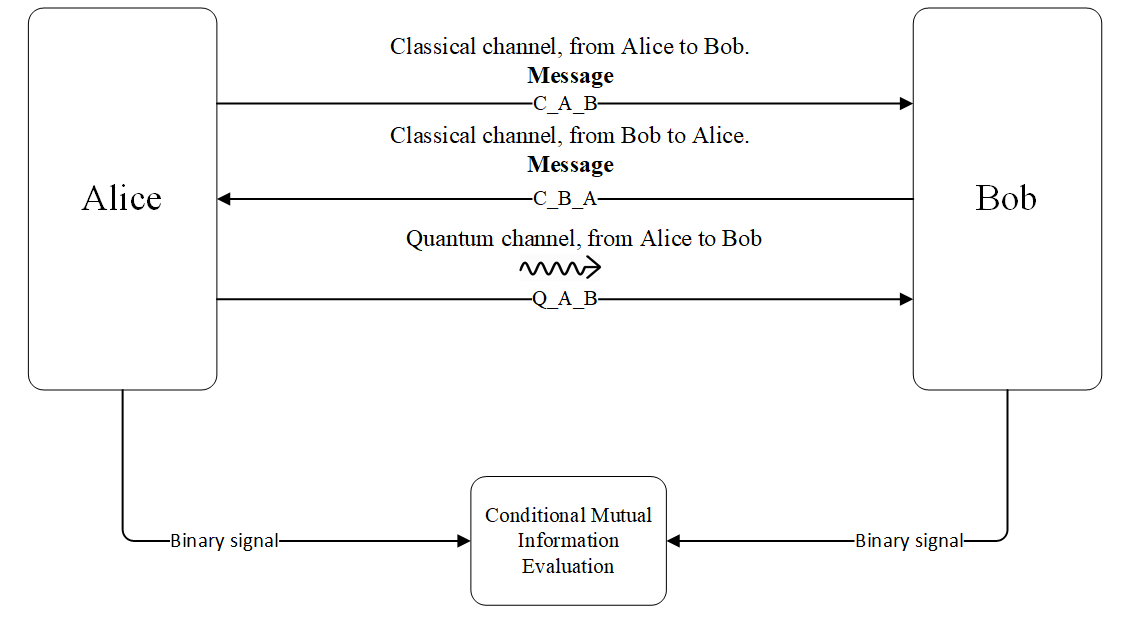
\includegraphics[width=1.0\textwidth, height=9cm]{./sdf/ot_with_discrete_variables/figures/Simulation_diagram_top.png}
	\caption{Simulation diagram at a top level}\label{toplevelsimulation}
\end{figure}

As one may see in figure \ref{toplevelsimulation} this simulation will have three top level blocks. Two of them are Alice and Bob and they are connected through two classical channels and one quantum channel. In addition, a third block will be performed in order to calculate the \textit{Mutual Information}. The mutual information (MI) between Alice and Bob is defined in terms of their join distribution.


\begin{enumerate}
  \item

  \begin{figure}[h]
	\centering
	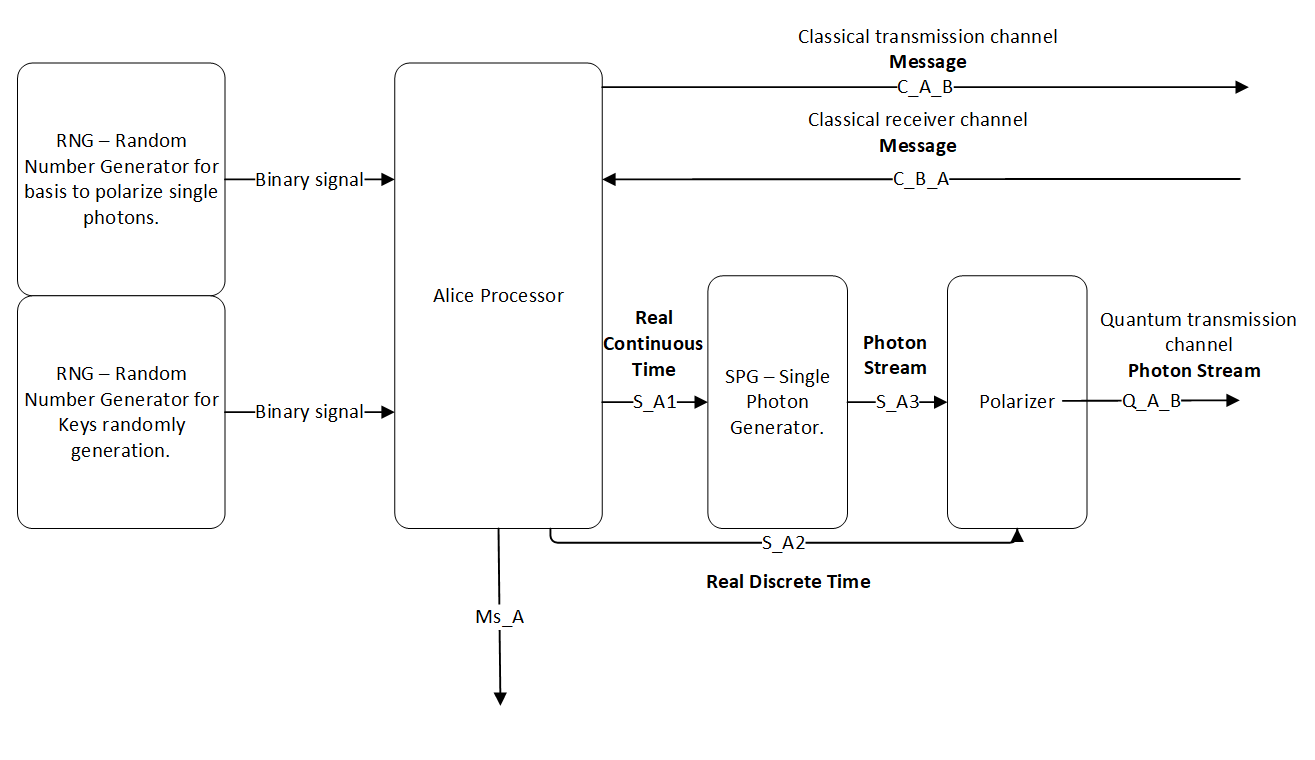
\includegraphics[width=1.1\textwidth, height=9cm]{./sdf/ot_with_discrete_variables/figures/Simulation_Alice.png}
	\caption{Simulation diagram - Alice's side}\label{simulationalice}
\end{figure}

    In figure \ref{simulationalice} one can observe a block diagram of the simulation at Alice's side. As it is shown in the figure, Alice must have two blocks for random number generation: one for basis generation in order to polarize the photons according this basis, and other for key random generation in order to have a random state to encode each photon. Furthermore, she has a Processor block for all logical operations: array analysis, hash function results validation, and others. This block also receives the start information, i.e. message size s, the expansion factor k and messages $m_{0}$ and $m_{1}$, as well as information from Bob, i.e sets $I_{0}$ and $I_{1}$, hash function results, and others. This block also must be responsible for send classical information to Bob. Finally, Processor block will also send a real continuous time signal to single photon generator, in order to generate photons according to this signal, and finally this block also sends to polarizer a real discrete signal in order to inform the polarizer which basis it should use. Therefore, she has two more blocks for quantum tasks: the single photon generator and the polarizer block which is responsible to encode the photons generated from the previous block and send them throughout a quantum channel from Alice to Bob.

    Finally, Alice's processor has an output to Mutual Information top level block, $Ms_{A}$.

  \item

  \begin{figure}[h]
	\centering
	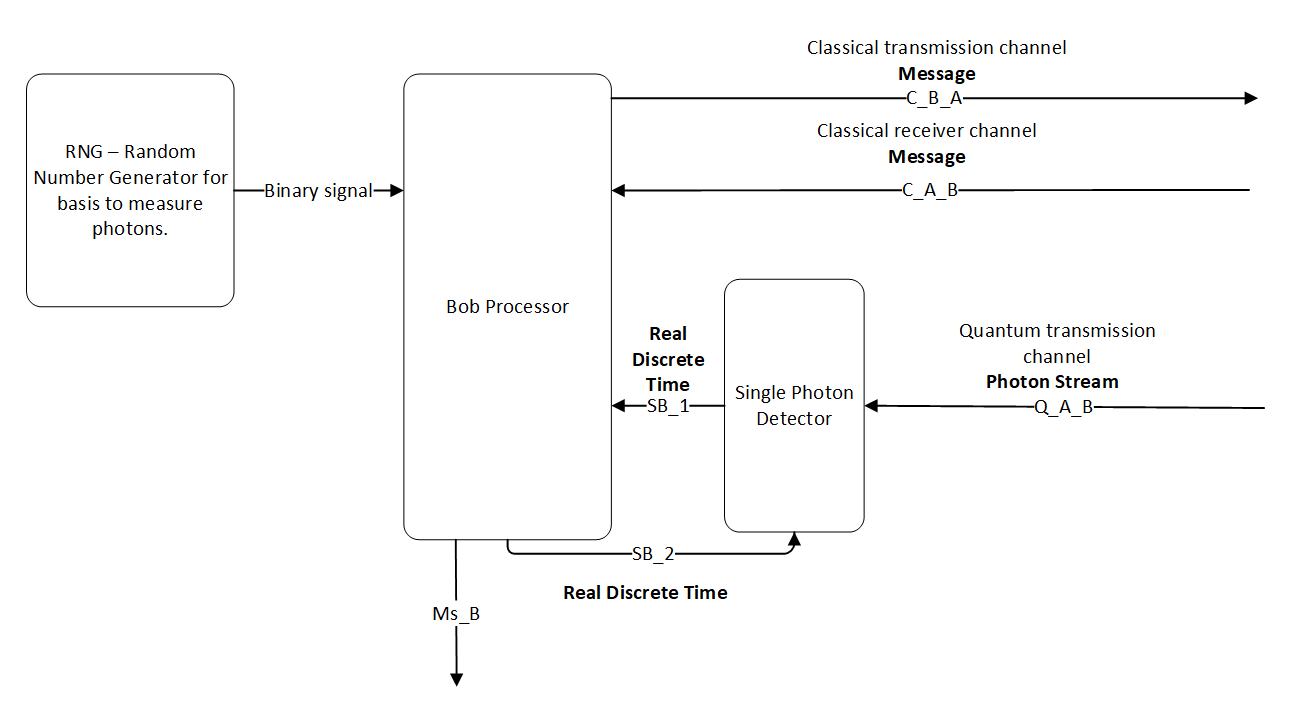
\includegraphics[width=1.1\textwidth, height=9cm]{./sdf/ot_with_discrete_variables/figures/Simulation_Bob.png}
	\caption{Simulation diagram - Bob's side}\label{simulationbob}
\end{figure}

    In figure \ref{simulationbob} one can observe a block diagram of the simulation at Bob's side. From this side, Bob only has one block for Random Number Generation which is responsible for randomly generate basis values which Bob will use to measure the photons sent by Alice throughout the quantum channel. Like Alice, Bob has a Processor block responsible for all logical tasks, i.e Hash function generation, analysing functions, etc. It receives information from Alice throughout a classical channel and a quantum channel but it sends information to Alice only throughout a classical channel. Furthermore, Bob has one more block for single photon detection which receives from processor block a real discrete time signal, in order to obtain the basis it should use to measure the photons.

    Finally, Bob's processor has an output to Mutual Information top level block, $Ms_{B}$.

  \item Mutual Information calculation
  \item
  \item
  \item
\end{enumerate}





\subsection{Experimental}
In figures \ref{quantumchannelcommunication1} and \ref{quantumchannelcommunication2} are presented the experimental setup to be performed in the lab. Starting with Alice's side and then Bob's side.

\begin{figure}[H]
	\centering 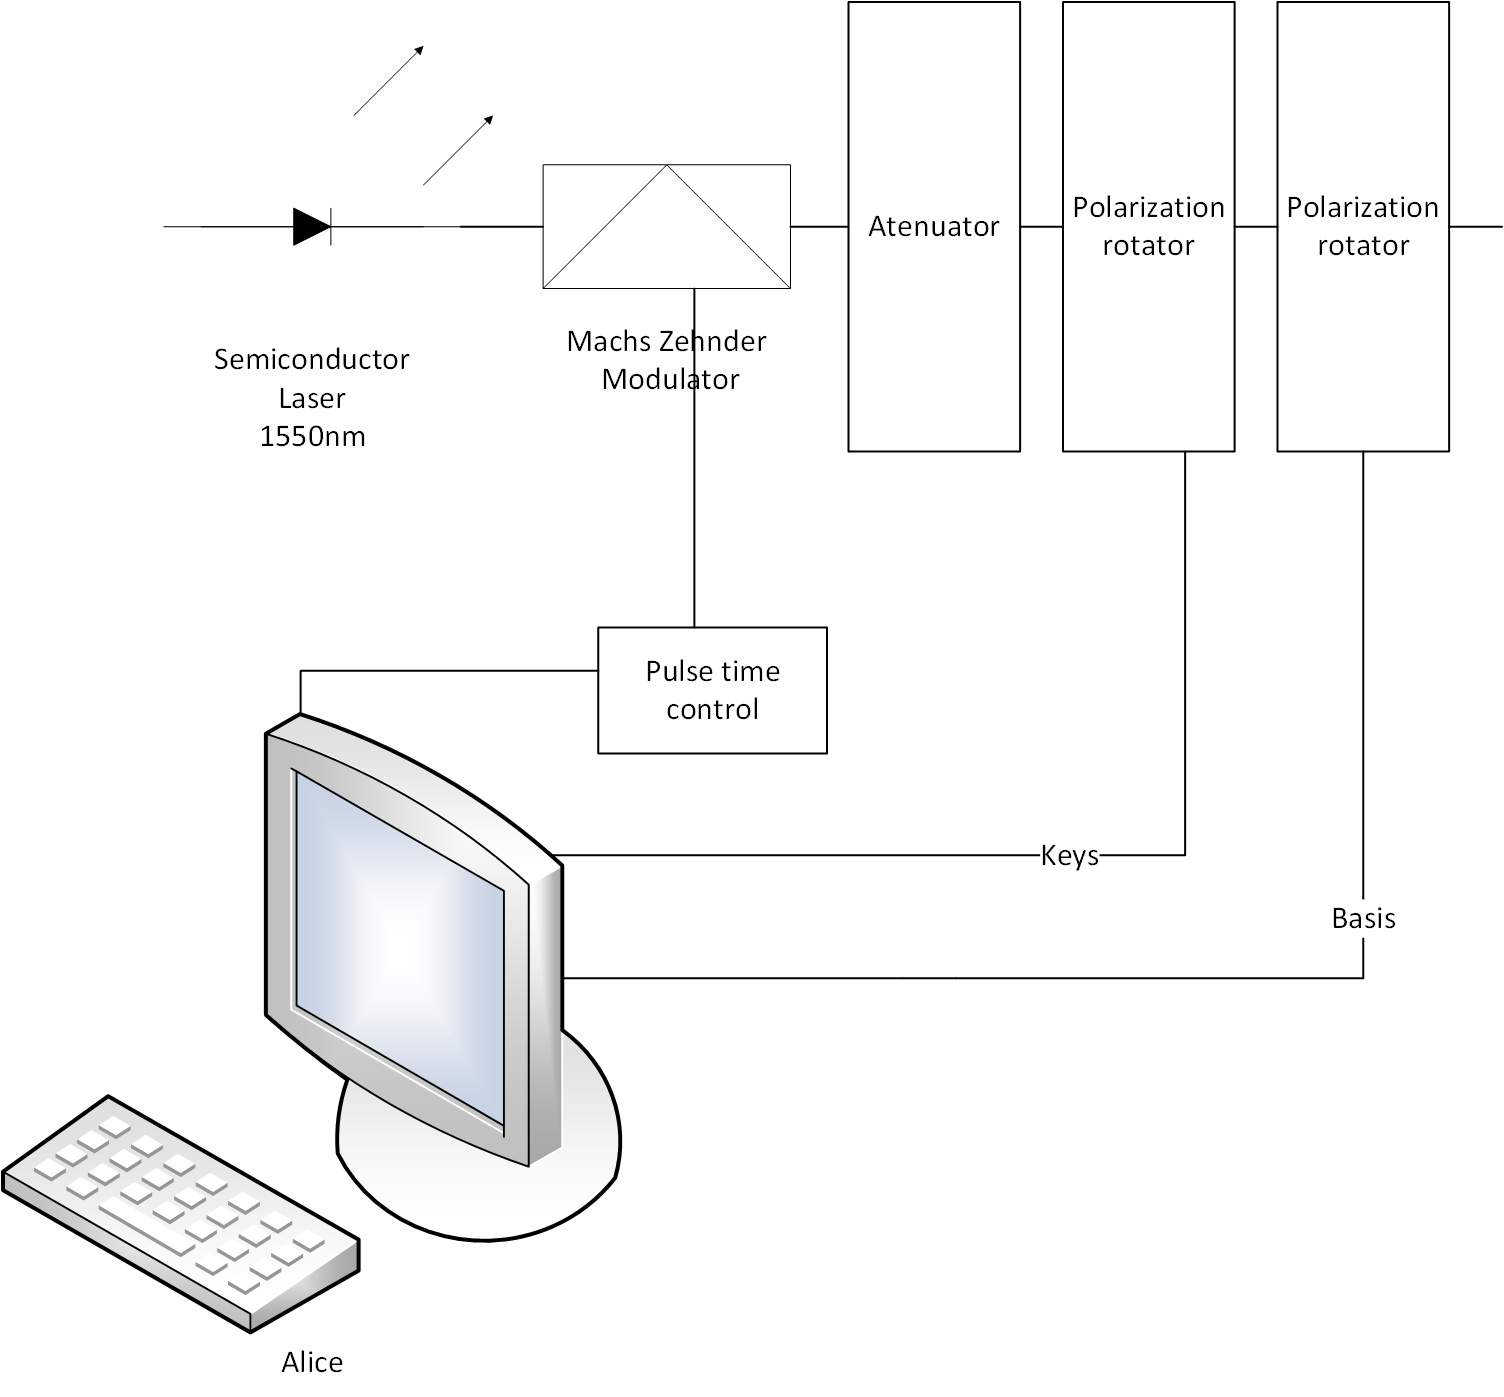
\includegraphics[width=0.8\textwidth,height=8cm]{./sdf/ot_with_discrete_variables/figures/OT_experimental_alice.png}
	\caption{Quantum communication diagram - Alice's side}\label{quantumchannelcommunication1}
\end{figure}

\begin{figure}[H]
	\centering 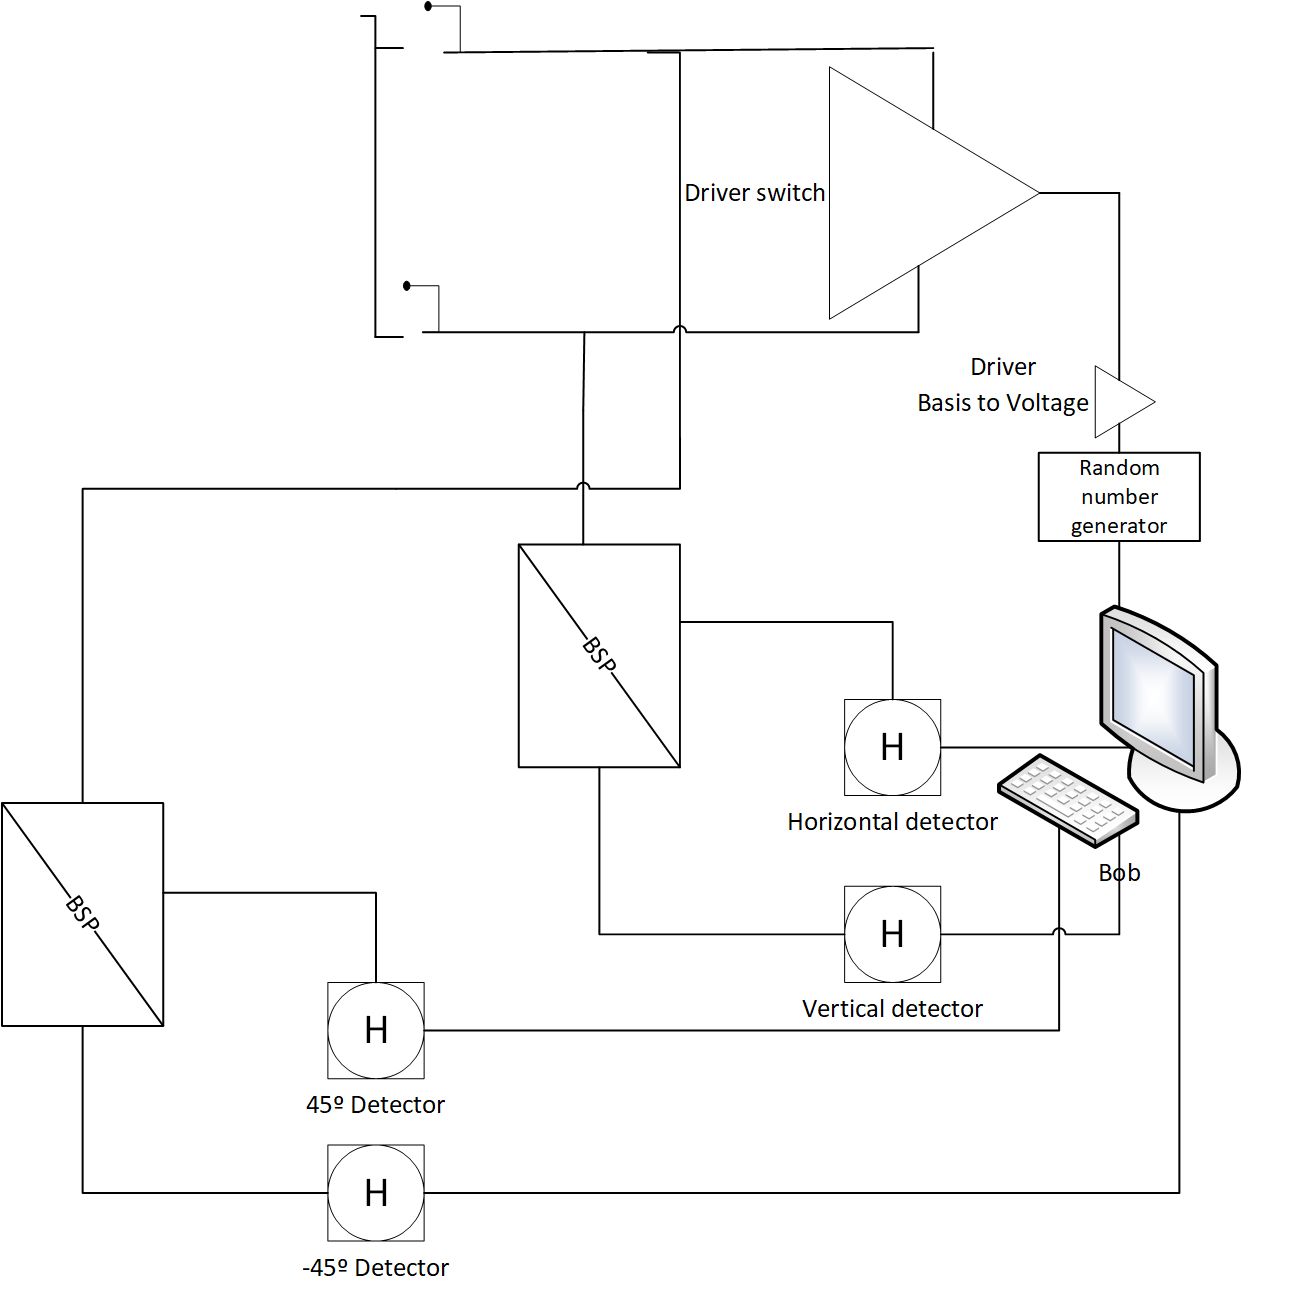
\includegraphics[width=0.8\textwidth,height=9cm]{./sdf/ot_with_discrete_variables/figures/OT_experimental_bob.png}
	\caption{Quantum communication diagram - Bob's side}\label{quantumchannelcommunication2}
\end{figure}

\bibliography{ot_with_discrete_variables}
